\section{Природные алгоритмы в настройке гиперпараметров}\label{Section:Performance}

Как уже было сказано, оптимизация гиперпараметров -- это поиск набора переменных, который позволит
алгоритму достичь более качественных результатов. Гиперпараметры обычно оказывают 
значительное влияние на успех алгоритмов машинного обучения. 
Когда требуется охватить большое пространство поиска, чтобы не застрять 
в локальном минимуме, и одновременно ограничить количество обучаемых 
моделей до приемлемого количества, при оптимизации гиперпараметров прибегают 
использованию более сложных алгоритмов, чем поиск по сетке или случайный поиск. 
В частности, возможно применений природных алгоритмов.

\subsection{Оценка производительности моделей}\label{Scorer}

Для оценки производительности некоторой обученной модели можно используют определенные метрики.

    \subsubsection{Матрица ошибок}

        Обнаружение спама в электронных письмах можно оценить с помощью
        различных показателей эффективности. Матрица ошибок используется для 
        визуализации работы алгоритмов и может быть определена как на Рисунке \ref{CM}.

        \begin{figure}[H]	
            \centering
            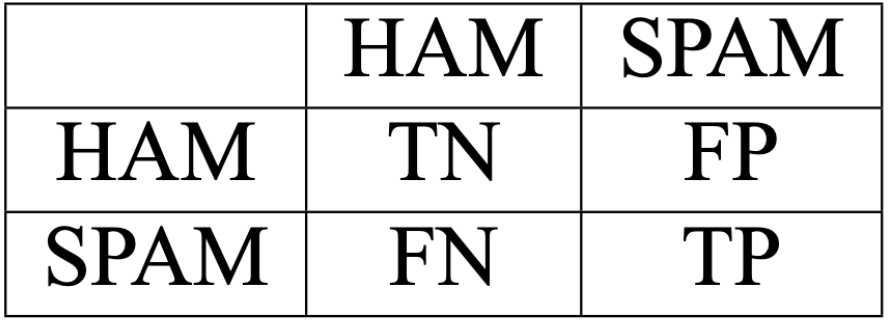
\includegraphics[width=40mm]{\pwd/table.png}
            \caption{Матрица ошибок}
            \label{CM}
        \end{figure}
        где:

        \begin{itemize}
            \item[-] TN = TrueNegative -- Письма, распознанные как письма;
            \item[-] FP = FalsePositive -- Спам-письма, распознанные как письма;
            \item[-] FN = FalseNegative -- Письма, распознанные как спам-письма;
            \item[-] TP = TruePositive -- Спам-письма, распознанные как спам-письма.
        \end{itemize}

    \subsubsection{Accuracy}
    
        Accuracy -- это отношение количества правильных прогнозов к общему количеству входных 
        выборок \cite{scikitMetrics}:
        
        \begin{equation}\label{eq11}
            Accuracy = {{(TN + TP)} \over{(TP + FN + FP + TN)}}
        \end{equation}
    
    \subsubsection{Recall}
    
        Recall описывает, сколько писем было правильно отнесено к спаму из 
        общего количества писем, распознанных как спам $(TP + FN)$ \cite{scikitMetrics}:

        \begin{equation}\label{eq12}
            Recall = {{TP} \over{(TP + FN)}}
        \end{equation}
    
    \subsubsection{Precision}
    
        Измерение precision заключается в доли верно идентифицированного 
        спама из всех спам-писем $(TP + FP)$ \cite{scikitMetrics}. Определяется 
        уравнением:

        \begin{equation}\label{eq13}
            Precision = {{TP} \over{(TP + FP)}}
        \end{equation}
    
    \subsubsection{F1-score}
    
        Оценка $F1$ может быть интерпретирована как средневзвешенное 
        значение precision и recall, где оценка $F1$ достигает своего лучшего 
        значения при 1 и худшего значения при 0 \cite{scikitMetrics}.
        Формула для оценки $F1$:

        \begin{equation}\label{eq14}
            F1 = {2 \times (precision \times recall) \over{(precision + recall)}}
        \end{equation}


\subsection{Переобучение}
Мы, люди, иногда склонны делать чрезмерные обобщения. К сожалению, 
машины могут оказаться в такой же ситуации. В контексте МО это называется 
\emph{переобучением}. 

Ограничение модели с целью ее упрощения и снижения риска переобучения 
называется \emph{регуляризацией} \cite{scikitBook}.

Тестирование модели на одних и тех же данных при выборе параметров является 
методологической ошибкой: модель, которая будет просто повторять метки 
образцов, которые она только что увидела, будет иметь идеальную оценку, но 
не сможет предсказать что-либо полезное на новых данных \cite{scikitTuning}. 

Чтобы решить эту проблему, еще одна часть набора данных может быть представлена ​​
как так называемый проверочный набор \emph{(validation set)}: обучение продолжается 
на обучающем наборе, после чего выполняется оценка на проверочном наборе, и 
когда эксперимент кажется успешным, окончательную оценку можно провести на 
тестовом наборе \cite{scikitCV}.

Однако, разбивая доступные данные на три набора, мы резко сокращаем количество 
выборок, которые можно использовать для изучения модели, и результаты могут 
зависеть от конкретного случайного выбора для пары наборов.

Решением этой проблемы является процедура \emph{перекрестной проверки} (сокращенно CV). 
Набор тестов по-прежнему должен храниться для окончательной оценки, но набор для 
проверки больше не нужен. В базовом подходе, называемом k-fold CV, 
обучающая выборка разбивается на k меньших наборов. Для каждого набора 
выполняется:

\begin{itemize}
    \item[-] Модель обучается с использованием $k - 1$ наборов в качестве обучающих данных;
    \item[-] Результирующая модель проверяется на оставшейся части данных (то есть 
    используется в качестве тестового набора для вычисления показателя 
    производительности).
\end{itemize}

Показатель производительности, полученный перекрестной проверкой, является 
средним из значений, вычисленных в цикле. Такой подход может быть дорогостоящим 
в вычислительном отношении, но не расходует слишком много данных.
